%% main file
%%


\documentclass[ebook,9pt,openany,final,french]{memoir}


\usepackage{babel}
\usepackage[utf8]{inputenc}

\usepackage{relsize}      % provide relative font size changes
\usepackage{underscore}   % remove special status of '_' in ordinary text
\usepackage{verbatim}     % improved verbatim environment
\usepackage{parskip}      % handle non-indented paragraphs "properly"
\usepackage{array}        % new column definitions for tables
\usepackage[normalem]{ulem}
\usepackage{color}        % define colors for strikeouts and underlines
\usepackage{amsmath}      % additional math symbols
\usepackage{mathrsfs}     % mathscr font
\usepackage{microtype}
\usepackage{xspace}
\usepackage{fixme}
\usepackage{lmodern}
\usepackage[T1]{fontenc}
\usepackage[pdftex, final]{graphicx}
\usepackage[pdftex,
            pdftitle={VADEMECUM FINANCE - Vincent CHAMBRIN},
            pdfsubject={},
            pdfcreator={Vincent CHAMBRIN},
            bookmarks=true,
            bookmarksnumbered=true,
            pdfpagelabels=true,
            pdfpagemode=UseOutlines,
            pdfstartview=FitH,
            linktocpage=true,
            colorlinks=true,
            linkcolor=blue,
            plainpages=false
           ]{hyperref}
\usepackage{memhfixc}     % fix interactions between hyperref and memoir
\usepackage{xstring}
\usepackage{caption}
\usepackage{amsfonts}
\usepackage{stmaryrd}
\usepackage{cite}
\usepackage{eurosym}
\usepackage{mathtools}

\usepackage{multirow}


%%--------------------------------------------------
%%  set page size, type block size, type block position

\setstocksize{19cm}{10.5cm}
\settrimmedsize{\stockheight}{\stockwidth}{*}
\setlrmarginsandblock{1cm}{1cm}{*} % Left and right margin
\setulmarginsandblock{1cm}{0.7cm}{*}  % Upper and lower margin


%%--------------------------------------------------
%%  set header and footer positions and sizes

\setheadfoot{\onelineskip}{2\onelineskip}
\setheaderspaces{*}{2\onelineskip}{*}

\setlength{\headheight}{0.5cm}
\setlength{\headsep}{0.5cm}
\setlength{\uppermargin}{1.6cm}
\setlength{\textheight}{16.5cm}
\setlength{\footskip}{0cm}
\setlength{\marginparsep}{0bp}
\setlength{\marginparpush}{0bp}
\setlength{\marginparwidth}{0bp}


%%--------------------------------------------------
%%  make miscellaneous adjustments, then finish the layout
\setmarginnotes{7pt}{7pt}{0pt}
\checkandfixthelayout


%%--------------------------------------------------
%%  create chapter style

\makechapterstyle{chapterStyle}{%
  \renewcommand{\beforechapskip}{\onelineskip}
  \renewcommand{\afterchapskip}{\onelineskip}
  \renewcommand{\chapternamenum}{}
  \renewcommand{\chapnamefont}{\chaptitlefont}
  \renewcommand{\chapnumfont}{\chaptitlefont}
  \renewcommand{\printchapternum}{\chapnumfont\thechapter\quad}
  \renewcommand{\afterchapternum}{}
}

%% Custom chapter title
\usepackage[explicit]{titlesec}
\titleformat{\chapter}[display]
  {\Large\centering\scshape}
  {\filcenter\chaptertitlename\Huge\thechapter}
  {0ex}
  {\titleline[c]{\titlerule[.4pt]}\vspace{1ex} #1}
  [{\vspace{1ex}\titleline[c]{\titlerule[.4pt]}}] 
  
\titlespacing*{\chapter}{0pt}{-15pt}{40pt}

\let\oldtitleline\titleline
\renewcommand{\titleline}{\oldtitleline*}
\setlength{\titlewidth}{0.75\textwidth}


\newcommand\normalchapterstyle{
  \titlespacing*{\chapter}{0pt}{-40pt}{10pt}
  \titleformat{\chapter}{\Large\textbf}{}{0pt}{}{}
  \titleformat{\section}{\large\textbf}{}{0pt}{}
  \titleformat{\subsection}{\normalsize\textit}{}{0pt}{}
}

%\makeatletter
%\def\thickhrulefill{\leavevmode \leaders \hrule height 1ex \hfill \kern \z@}
%\def\@makechapterhead#1{%
%  \vspace*{10\p@}%
%  {\parindent \z@ \centering \reset@font
%        {\Huge \scshape \thechapter}
%        \par\nobreak
%        \vspace*{15\p@}%
%        \interlinepenalty\@M
%        \setlength{\arrayrulewidth}{1pt}
%        \begin{tabular}{@{\qquad}c@{\qquad}}
%          \hline
%          \\
%          {\Huge \bfseries #1\par\nobreak} \\
%          \\
%          \hline
%        \end{tabular}
%    \vskip 30\p@
%  }}
%\def\@makeschapterhead#1{%
%  \vspace*{10\p@}%
%  {\parindent \z@ \centering \reset@font
%        {\Huge \scshape \vphantom{\thechapter}}
%        \par\nobreak
%        \vspace*{15\p@}%
%        \interlinepenalty\@M
%        \setlength{\arrayrulewidth}{2pt}
%        \begin{tabular}{@{\qquad}c@{\qquad}}
%          \hline
%          \\
%          {\Huge \bfseries #1\par\nobreak} \\
%          \\
%          \hline
%        \end{tabular}
%    \vskip 100\p@
%  }}


%%--------------------------------------------------
%%  create page styles

\makepagestyle{pageStyle}
\makeevenhead{pageStyle}{\thepage}{\textsc{VADEMECUM FINANCE}}{}
\makeoddhead{pageStyle}{}{\textsc{VINCENT CHAMBRIN}}{\thepage}
%\makeevenfoot{pageStyle}{\leftmark}{}{\thepage}
%\makeoddfoot{pageStyle}{\leftmark}{}{\thepage}

\makeatletter
\makepsmarks{pageStyle}{%
  \let\@mkboth\markboth
  \def\chaptermark##1{\markboth{##1}{##1}}%
  \def\sectionmark##1{\markboth{%
    \ifnum \c@secnumdepth>\z@
      \textsection\space\thesection
    \fi
    }{\rightmark}}%
  \def\subsectionmark##1{\markboth{%
    \ifnum \c@secnumdepth>\z@
      \textsection\space\thesubsection
    \fi
    }{\rightmark}}%
  \def\subsubsectionmark##1{\markboth{%
    \ifnum \c@secnumdepth>\z@
      \textsection\space\thesubsubsection
    \fi
    }{\rightmark}}%
  \def\paragraphmark##1{\markboth{%
    \ifnum \c@secnumdepth>\z@
      \textsection\space\theparagraph
    \fi
    }{\rightmark}}}
\makeatother

\aliaspagestyle{chapter}{pageStyle}

%%--------------------------------------------------
%%  set heading styles for main matter
\newcommand{\beforeskip}{-.7\onelineskip plus -1ex}
\newcommand{\afterskip}{.3\onelineskip minus .2ex}

\setbeforesecskip{\beforeskip}
\setsecindent{0pt}
\setsecheadstyle{\large\bfseries\raggedright}
\setaftersecskip{\afterskip}

\setbeforesubsecskip{\beforeskip}
\setsubsecindent{0pt}
\setsubsecheadstyle{\large\bfseries\raggedright}
\setaftersubsecskip{\afterskip}

\setbeforesubsubsecskip{\beforeskip}
\setsubsubsecindent{0pt}
\setsubsubsecheadstyle{\normalsize\bfseries\raggedright}
\setaftersubsubsecskip{\afterskip}

\setbeforeparaskip{\beforeskip}
\setparaindent{0pt}
\setparaheadstyle{\normalsize\bfseries\raggedright}
\setafterparaskip{\afterskip}

\setbeforesubparaskip{\beforeskip}
\setsubparaindent{0pt}
\setsubparaheadstyle{\normalsize\bfseries\raggedright}
\setaftersubparaskip{\afterskip}


%%--------------------------------------------------
%%  set footnote style
\footmarkstyle{\smaller#1) }

%%--------------------------------------------------
% set style for main text
\setlength{\parindent}{0.3cm}
%\setlength{\parskip}{1ex}
%\setlength{\parskip}{0ex}
\setlength{\parskip}{\onelineskip}
\setlength{\partopsep}{-1.5ex}

%%--------------------------------------------------
%% set global styles that get reset by \mainmatter
\newcommand{\setglobalstyles}{
  \counterwithout{footnote}{chapter}
  \counterwithout{table}{chapter}
  \counterwithout{figure}{chapter}
  \renewcommand{\chaptername}{}
  \renewcommand{\appendixname}{Annexe }
}

%%--------------------------------------------------
%% set section numbering limit, toc limit
\maxsecnumdepth{subparagraph}
\setcounter{tocdepth}{1}



% Non French Words
\newcommand{\nfw}[1]{\emph{#1}\xspace}


\makeindex


%%--------------------------------------------------
%% fix interaction between hyperref and other
%% commands
\pdfstringdefDisableCommands{\def\smaller#1{#1}}
\pdfstringdefDisableCommands{\def\textbf#1{#1}}
\pdfstringdefDisableCommands{\def\raisebox#1{}}
\pdfstringdefDisableCommands{\def\hspace#1{}}


\begin{document}
\chapterstyle{chapterStyle}
\pagestyle{pageStyle}

\frontmatter


\thispagestyle{empty}

\vfill

\vspace*{1cm}

\begin{center}
{\fontsize{30}{40}\selectfont\raisebox{-0.3 em}{\fontsize{50}{60}\selectfont\/V}{\kern -0.3em}AD\raisebox{-0.2 em}{E}\raisebox{0.0 em}{M}\raisebox{-0.2 em}{E}CU\raisebox{0.0 em}{M}}
\end{center}

\vspace{2cm}

\begin{center}
{\fontsize{25}{30}\selectfont \textsc{FINANCE}}
\end{center}

\vspace{2cm}

\begin{center}
  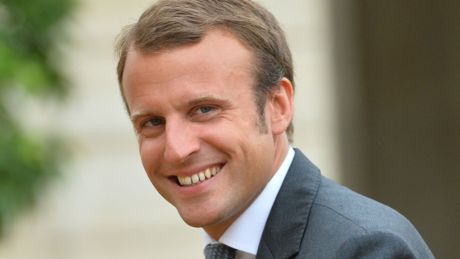
\includegraphics[scale=0.45]{assets/cover}
\end{center}


\vfill


\newpage

\newpage


\cleardoublepage

\thispagestyle{empty}

\vspace*{\fill}


\begin{center}
Ce produit est sponsorisé par P.\/ Gilquin SAII (société à irresponsabilité illimitée). \\
Pour toute erreur ou imprécision, veuillez donc vous adressez à H.\/ Gissler.
\end{center}


\vspace*{\fill}

\noindent
Ce qui va suivre peut heurter la sensibilité de certaines personnes. 
\\
En conséquence, il ne faut absolument pas tenter de reproduire ou d'imiter le contenu  
de ce programme. \\
Avant d'aller plus loin, veuillez vérifier que vous êtes bien aptes à lire 
un document traitant de la finance d'entreprise. 
En cas de doutes, demandez l'avis de votre médecin.

\vspace{2em}

\begin{center}
© 2018, Vincent Chambrin. 
\end{center}

\newpage



\newpage
\let\oldleftmark=\leftmark
\renewcommand{\leftmark}{Table des matières}

\setcounter{tocdepth}{4}
%\tableofcontents

\pagebreak
\let\leftmark=\oldleftmark

\mainmatter
\setglobalstyles


\chapter{Cash et Résultat \\ tu ne confondra point}

\chapterprecishere{``Tout le monde peut faire une erreur [...]; mais cette 
erreur ne devient une faute que si vous refusez de la corriger''\par\raggedleft--- Mitth'raw'nuruodo}

Il est 8h, je viens d'arriver au boulot.
Les vacances approchent, la plupart des gens sont sur les nerfs. 
Je me dirige vers la salle de repos pour me préparer un thé. 
La machine à café étant en panne depuis presque deux semaines, 
nous avons recours à une bouilloire pour faire chauffer l'eau.
En m'approchant, j'entends que le volume dans la salle n'est 
certainement pas reposant. C'est Bernard, le commercial, 
qui rage sur la machine qui n'a toujours pas été réparée. 
Les personnes présentent ne savent plus où se mettre... 
Prenant mon courage à deux mains, je décide d'essayer de 
l'écouter pour qu'il se calme.
\begin{itemize}
  \item "Un problème Bernard ? "
  \item "Bah oui ça fait chier la machine qui est toujours en 
  panne ça fait trois semaines !"
\end{itemize}
Étant diplomate, je décide de ne pas lui faire remarquer que 
la machine n'est en panne que depuis seulement deux semaines, et pas 
trois.
\begin{itemize}
  \item "Oui, je sais. Mais t'inquiètes elle va bientôt être 
  réparée, c'est sûre."
  \item "Et bah non justement, j'ai été voir le patron et il 
  a dit qu'on avait pas l'argent pour réparer la machine, t'imagines !"
\end{itemize}
C'est à ce moment là que j'ai décidé d'appliquer la méthode DG, 
qui consiste à écouter la personne râler jusqu'à la dernière 
goutte. On peut alors discuter plus calmement. 
Il continua en affirmant que c'était scandaleux, qu'on avait 
demandé aux commerciaux d'augmenter les ventes d'au 
moins 5\%, et que c'est ce qu'ils avaient fait et même 
mieux.
\begin{itemize}
  \item "7\% on a fait, 7\% tu te rends compte !"
\end{itemize}
Il me demanda si j'avais assisté à la présentation des 
résultats de l'entreprise hier, ce à quoi je répondis oui; et 
continua en m'expliquant que le chiffre d'affaires et le 
résultat avaient augmentés comme prévu. 
Il ne comprenait donc pas pourquoi on n'avait pas l'argent 
pour réparer cette "foutue" machine à café. 
Il estimait que lui et les autres commerciaux méritaient 
d'être mieux traités que cela après les efforts qu'ils avaient 
fait.

Il faut dire que la présentation de la veille ne présentait 
que les aspects positifs des résultats de la société, et 
ce en partie pour ne pas démoraliser les troupes qui avaient 
fait des efforts mais également peut-être par lâcheté et 
habitude du manager, un ancien d'Audencia, qui a l'habitude de 
ne montrer que ce qui est plaisant. 
Le résultat de la boîte s'est en effet amélioré mais pas sa 
trésorerie, ce qui explique qu'il n'y ai plus d'argent pour 
le café... 

Pour comprendre ce qu'il se passe, il faut étudier trois 
documents comptables: le compte de résultat, le bilan, et le 
tableau des flux de trésorerie. 
Les normes françaises imposent aux entreprises de soumettre 
les deux premiers à l'Etat.

Le compte de résultat est un document dont le but est de 
refléter l'activité de la société sur une année (un \emph{exercice});
le bilan est là quant à lui pour 
présenter ce que possède la société, en terme d'argent mais 
également de biens matériels, et comment elle l'utilise.

Un exemple de ces documents est présenté un peu plus en détails en annexe.

Le compte de résultat est découpé en trois grandes parties : 
la partie relative au résultat d'exploitation, celle relative 
au résultat financier et enfin une dernière partie sur le 
résultat exceptionnel. La somme de ces trois résultats forme 
le résultat de l'exercice.

Le bilan est découpé en deux parties : l'actif (ce que j'ai) 
et le passif (mes ressources, i.e. ce que je dois).
Autrement dit, le bilan présente les ressources de l'entreprise 
et comment elle les utilise; le bon sens Pornicais impose donc que 
le passif soit égal à l'actif\footnote{On parle aussi de bon sens paysan (BSP)}.

L'une des notions les plus importantes est que le compte 
de résultat ne représente pas du cash. En effet, sont 
enregistrés dans le compte de résultat toutes les factures dès 
leur émission et tous les achats dès leur réception : le 
compte de résultat ne prend pas en compte le paiement effectif. \\
\hspace*{\parindent}Une autre raison est qu'il est inscrit dans le compte de 
résultat les dotations aux amortissements : dès que j'achète un bien 
d'une valeur supérieure à 500\euro\/, je ne le fais pas passer 
entièrement dans le compte de résultat mais je l'étale sur 
plusieurs exercices (cela permet de prendre en compte le fait 
que j'utilise ce bien sur plusieurs exercices et qu'il perd de sa 
valeur).

Le tableau des flux de trésorerie permet de passer du 
résultat au cash.

\begin{table}[h]
\renewcommand{\arraystretch}{1.2}
\footnotesize
\centering
\begin{tabular}{|l|c|}
\hline                                                                                                                                                                
  CAF    & 120 \\
\hline                                                                                                                                                              
  Variation du BFR  & (20) \\
\hline                                                                                                                                                              
  Cash Flow d'Exploitation & 100 \\
\hline  
  Flux de trésorerie d'investissement & 10 \\
\hline     
Cash Flow Libre & 110 \\                                                                                                                                                                                                                                                                                              
\hline                                                                                                                                                                
Flux de trésorerie de financement & (120) \\
\hline     
Variation de trésorerie & (10) \\                                                                                                                                                                                                                                                                                              
\hline  
Trésorerie au début de l'exercice & 5 \\                                                                                                                                                                                                                                                                                              
\hline  
Trésorerie à la fin de l'exercice & (5) \\                                                                                                                                                                                                                                                                                              
\hline  
\end{tabular}
\label{tftex1}
\caption{Tableau des flux de trésorerie simplifié}
\end{table}

Les délais de paiement des clients et des fournisseurs 
introduisent la notion de besoin en fonds de roulement (BFR) 
et de fonds de roulement. Concrètement, le BFR est la 
trésorerie qu'il me faut à l'avance pour pouvoir payer mes 
fournisseurs avant de recevoir le paiement de mes clients.
Son expression est la suivante:
\begin{equation*} \label{eq:BFR}
\mathrm{BFR} = \text{Stocks} + \text{Créances clients} - \text{Dettes fourniseurs}
\end{equation*}
Le fond de roulement est le cash disponible pour combler le 
BFR. Il doit donc être supérieur au BFR pour éviter de devoir 
s'endetter.
\[
\mathrm{FR} = \text{Capitaux permanents} - \text{Actifs immobilisés}
\]
où les capitaux permanents sont la somme des capitaux propres et des dettes à moyen et long terme.

Ces deux quantités sont calculables à partir du bilan.

Comme on peut le voir pour notre société, c'est la variation 
du besoin en fonds de roulement qui fait passer la trésorerie 
dans le rouge. Les ventes ont certes augmentées, mais comme 
le besoin en fonds de roulement a lui aussi augmenté la 
situation financière s'est dégradée. 
L'augmentation du BFR peut avoir pour origine: 
\begin{itemize}
 \item une augmentation des stocks;
 \item une augmentation des créances clients;
 \item une diminution de la dette fournisseurs (e.g. on paye plus vite qu'auparavant);
 \item une combinaison des trois.
\end{itemize}
Ici, c'est probablement l'augmentation des ventes qui a entraîné une augmentation des créances.

Cette exemple montre deux choses importantes:
\begin{itemize}
 \item il est important de maîtriser sont BFR (composantes par composantes);
 \item le résultat ne se traduit pas immédiatement en cash à cause des délais de paiement.
\end{itemize}

L'évaluation de la santé d'une société peut se faire de 
plusieurs manières. En comptabilité analytique, on utilise 
les soldes intermédiaires de gestion (c.f.\/ table \ref{table:sig} annexe \ref{chapter:sig}). 
En analyse financière, on va utiliser d'autres indicateurs que l'on peut 
construire à partir des documents comptables. 

Il est possible de faire une analyse très rapide en utilisant seulement trois indicateurs 
que l'on trouve au début, au milieu et à la fin du compte de résultat. Ces indicateurs 
comptables et leurs équivalents financiers sont présentés dans la table \ref{table:3indicateurs}.

\begin{table}[h]
\renewcommand{\arraystretch}{1.2}
\footnotesize
\centering
\begin{tabular}{|c|c|c|}
\hline
  Comptable & Financier & Sens \\                                                                      
\hline                                                                                                      
  CA & VA & Puissance \\                                                                    
\hline                                                                                                      
  REX & EBE & Moteur \\                                                                              
\hline                                                                                                          
  RNS & CAF & Développement \\                                                                                         
\hline                                                                                                      
\end{tabular}                                                                                                                                                                                                       
\caption{Analyse en 3 indicateurs}       
\label{table:3indicateurs}                                                    
\end{table}

Pour finir ce chapitre et à nouveau appuyer sur le fait que le \textsc{cash} est différent 
du résultat, nous ajouterons simplement que chaque année, une part non négligeable des entreprises 
qui sont dissoutent ont pourtant un résultat positif (mais sont à cours de \textsc{cash})...


\chapter{Un investissement rentable ?}


\chapterprecishere{``Un tiens vaut mieux que deux tu l'auras.''\par\raggedleft--- \textup{Le Petit Poisson et le Pêcheur}, La Fontaine}

Gérard, fidèle employé de notre petite société de
fabrication est fatigué de travailler sur une machine qui n'est 
plus à la pointe de la technologie. 
Voulant améliorer la situation, il décide de faire des 
recherches et finit par trouver une machine qui permettrait de 
produire autant et pour moi cher.
En plus de rendre la vie des travailleurs plus agréable, 
cette machine pourrait donc également permettre de faire 
des économies. \\
\hspace*{\parindent}Comme Gérard sait bien que le patron est souvent occupé, 
il décide de se construire un petit dossier pour appuyer son idée.
Il fait ses calculs et en déduit que l'investissement serait 
rentable en moins de 5 ans. \\
\hspace*{\parindent}Fier comme un bar-tabac, 
il court donc voir son patron pour lui 
soumettre l'idée. Il lui montre tout son petit dossier: la 
fiche technique de la machine, le coût de l'investissement 
et les économies qu'il va pouvoir réaliser chaque année.
Le patron, qui n'est pas né de la dernière pluie, sait que 
tout n'est pas si simple. Il suspecte que le calcul de 
son employé ne soit pas tout à fait juste. 
Cependant, comme il ne veut pas se mettre ses employés à dos, 
il décide de renvoyer le poisson vers le monsieur finance 
de l'entreprise. Après tout, ce dernier n'est déjà pas très apprécié 
par la majorité des employés, autant que ce soit lui qui 
annonce les mauvaises nouvelles.
\begin{itemize}
  \item "Oui, ça pourrait être intéressant, va donner ça à 
  Francis qu'il nous dise si c'est faisable"
  \item "Ok chef !"
\end{itemize}
\hspace*{\parindent}L'employé va alors voir le comptable, 
frappe à la porte de son bureau et fini par être accueilli par le 
comptable qui visiblement est dérangé (il était probablement 
en train d'effectuer son activité favorite, enregistrer des 
pièces comptables).
Gérard, voulant alors s'attribuer tout le mérite, s'adresse 
au comptable comme suit \\
\begin{itemize}
  \item "J'ai réfléchi à un investissement qui pourrait nous faire 
    économiser pas mal d'argent et le chef m'a dit de venir vous apportez ça,
	voilà en faite il s'agirait..."
  \item "Posez ça sur mon bureau je regarderais plus tard", 
    dit le comptable pour couper court à Gérard, voyant que 
    ce dernier allait probablement s'étendre en explications.
\end{itemize}
\hspace*{\parindent}Ce dernier, ne voulant pas risquer d'énerver le comptable, 
déposa son petit dossier sur le bureau et partit en se disant 
que tout allait aller comme sur des roulettes.
\hspace*{\parindent}Quelques jours plus tard, n'ayant pas de nouvelles,
Gérard va voir le comptable pour lui en demander. 
Il ressort de son bureau quelques minutes plus tard, bien 
énervé: le comptable a rejeté son idée ! 


Pour comprendre comment deux personnes sont arrivés 
à des conclusions différentes, il faut étudier la façon 
dont ils ont chacun fait leurs calculs.

Gérard, lui, a décidé de voir les choses simplement: le 
coût d'achat et de mise en service de la nouvelle machine 
serait de 100 k\euro\/; cette dernière permettrait sur 5 ans 
d'économiser 24 k\euro\/ par an. Au final, 
\[ 5 \times 24 - 100 = 20 > 0 \]
donc d'après Gérard le projet est rentable.

Le financier, quant à lui, sait que ce n'est 
cependant pas aussi simple que cela ! 
Lorsqu'il a fait son calcul, ce dernier a pris en compte 
le fait que $1$ euro dans 5 ans ce n'est pas $1$ euro aujourd'hui. 
Pour montrer cela, nous allons prendre l'exemple simple d'un placement à 
la banque. Supposons que je place en banque $x$ euros. 
Chaque année, la banque va me reverser $\alpha$ \% d'intérêts.
Ainsi, à l'issue de la première année, je n'aurais plus $x$ 
euros en banque mais $x \times (1+\alpha)$, quantité 
que nous appellerons $F_1$. 
\hspace*{\parindent}Ainsi, après seulement une année à la banque, 
j'ai déjà plus d'argent qu'au départ !
Si je laisse cet argent à la banque, et que les taux restent 
constant, je gagnerais chaque année une certaine somme tel que:
\[ F_n = x \times (1+\alpha)^n \]
Ceci montre bien qu'$1$ euro dans 5 ans, ce n'est pas $1$ euro 
aujourd'hui.
On peut évidemment faire autre chose de cet argent 
(ce n'était qu'un exemple), mais dans 
tous les cas, on peut espérer qu'il nous rapporte. 
Ceci implique qu'il est nécessaire "d'actualiser" les 
flux de trésorerie futurs pour faire un calcul plus juste.

La formule précédente nous permet d'estimer la valeur future 
de notre argent. En l'inversant, on peut calculer l'équivalent 
aujourd'hui d'un montant que l'on recevrait dans le futur.
\[ F_0 = \frac{F_n}{(1+\alpha)^n} \]
Dans cette formule, $\alpha$ est appelé le \emph{taux 
d'actualisation}, il permet d'actualiser la valeur d'une somme future.
On est alors en mesure de ré-estimer le coût de notre 
investissement.

La taux d'actualisation est en général pris égal au \emph{WACC} (\textit{weighted average cost of capital}, ou 
CMPC en français, coût moyen pondéré du capital).
Ce dernier se calcul de la manière suivante:
\begin{equation*}
\label{eq:WACC}
\mathrm{WACC} = \frac{C_p R + D_f I (1- t_i) }{C_p + D_f}
\end{equation*}
Avec:
\begin{itemize}
  \item $C_p$, les capitaux propres;
  \item $R$, le coût des capitaux propres, i.e.\ la rentabilité attendue par les actionnaires;
  \item $D_f$, les dettes financières;
  \item $I$, les intérêts des dettes financières;
  \item $t_i$, le taux d'imposition.
\end{itemize}

Moralement, ce quotient correspond au taux d'actualisation 
qui permet de satisfaire les investisseurs et de payer les 
intérêts des dettes; ces derniers sont coefficientés 
par le taux d'imposition car les intérêts font diminuer 
le résultat et donc l'impôt payé (ils sont en quelques sortes 
déductibles d'impôts).

Par exemple, pour $\alpha = 5\%$, on obtient.

\begin{table}[h]
\small
\centering
\begin{tabular}{|l|c|c|c|c|c|c|}
\hline
 Année & 0 & 1 & 2 & 3 & 4 & 5 \\
 Flux  & -100 & 24 & 24 & 24 & 24 & 24 \\
 Actualisé & -100 & 22,86 & 21,77 & 20,73 & 19,74 & 18,80 \\
 Cumul & -100 & -77,14 & -55,37 & -34,64 & -14,90 & 3,91 \\
\hline
\end{tabular}
\caption{Flux de trésorerie actualisé}
\end{table}

On se rend compte que ce calcul est tout de suite moins 
avantageux pour ce qui est de la rentabilité du projet: 
le ROI est ici un peu en dessous des 4\%, ce qui est 
assez faible.

La formule utilisé pour actualiser nos flux de trésorerie 
reste cependant un peu simpliste: elle suppose par exemple 
que le taux d'actualisation reste constant au cours du temps 
ce qui n'est pas réellement le cas. 
C'est pourquoi l'on effectue en général les calculs avec 
différents taux d'actualisation, pour voir à quel point 
l'investissement est intéressant. 
On s'intéresse en 
particulier à la valeur du taux d'actualisation, le TRI, qui 
annule les bénéfices. Plus le TRI est élevé, plus 
l'investissement est rentable.

Attention cependant, il est parfois préférable d'avoir 
un TRI relativement faible mais sur un projet d'une durée 
courte, plutôt qu'un TRI élevé mais sur un temps beaucoup 
plus long.

Ici, le calcul donne un TRI d'environ 6,4\%. 
Le projet a probablement été rejeté car cette valeur est 
inférieure au WACC de la société.




\chapter{Une activité indésirable ?}

\chapterprecishere{``La qualité !''\par\raggedleft--- Un membre de l'option Finance}

Je viens d'être embauché dans une petite entreprise de 
fabrication en tant qu'ingénieur qualité. Cette société 
familiale utilise ses nombreuses machines pour fabriquer 
du mobilier métalique et d'autres pièces de A à Z. \\
\hspace*{\parindent}En plus des machines de découpage et de pliage et des postes  
de soudage et de peinture, la société possède une grenailleuse :
il s'agit d'une machine capable d'envoyer sur les pièces du 
sable à haute vitesse pour éliminer les dépôts de rouille ou 
enlever une couche de peinture. \\
\hspace*{\parindent}Cette activité est la bête noire des employés car elle est 
extrêmement pénible. On commence par remplir un réservoir de 
grenaille (que l'on ramasse à même le sol), puis on 
enfile un scaphandre de projection et on projette la grenaille 
sur les pièces à l'aide d'une lance ! \\
\hspace*{\parindent}La machine étant viellisante, son efficacité a diminuée. 
De plus, le scaphandre de protection n'est plus tout à fait 
hermétique et la machine fait beaucoup de bruit ce qui rend 
le travail d'autant plus difficile à supporter. \\
\hspace*{\parindent}Pire encore, le comptable de la société est perturbé dans son 
travail d'enregistrement des pièces comptables par le bruit de 
la grenailleuse. Les finances de l'entreprise sont toujours 
justes, la société ayant fait le choix de la qualité sur la 
quantité, les clients se font rares...\footnote{Les clients 
sont néanmoins en général très satisfait du travail de la 
société.} \\ 
\hspace*{\parindent}Le comptable décide donc de faire des calculs pour voir si on 
ne pourrait pas faire des économies. A sa grande surprise, il 
découvre que le grenaillage est l'une des activités les moins 
rentables, à la limite de faire perdre de l'argent.
\begin{itemize}
 \item "Il faut qu'on arrête ça", se dit-il alors.
\end{itemize}
Ni une ni deux, le comptable sort alors de son bureau,
grimpe les escaliers, cours vers le bureau du patron. 
Il rentre dans le bureau tout essoufflé, il est peu habitué 
à faire du sport. 
\begin{itemize}
  \item "Chef, il faut qu'on parle du grenaillage"
\end{itemize}
Le chef, bien au courant de ce qu'il se passe dans son atelier, 
de lui répondre: "Oui oui je sais, il faut réinvestir dans la 
machine!".
Le financier tombe alors des nues puisque le patron vient de 
proposer exactement l'inverse de ce qu'il voulait suggérer.


Avant d'aller plus loin, il faut comprendre comment le 
comptable est arrivé à la conclusion que l'activité n'était pas 
rentable: nous allons pour cela faire un calcul de marge.

On peut regrouper les charges en 3 grandes catégories: 
\begin{itemize}
  \item les charges variables, liées au volume d'activité;
  \item les charges fixes spécifiques, ne dépendent pas du volume 
        d'activité mais disparaîtraient si on cessait l'activité;
  \item les charges communes, ne sont pas liées à une activité particulière.
\end{itemize}

Pour l'activité de grenaillage, l'entreprise achète chaque année 10 kg de grenailles 
à 60\euro\/ le kilo pour compenser les pertes. La fiche technique de la grenailleuse 
affiche un fonctionnement nominal sur du 400 V - 32 A. 
La prestation est facturée à l'heure, le tarif est fixé à 50\euro\/ l'heure. \\
Le comptable commence donc ses calculs. 
La machine consomme 12,8 kW; en prenant un coût de l'électricité à 14 centimes du kWh, 
on obtient 1,80\euro\/ par heure. En considérant que c'est la seule charge variable, 
on obtient une marge sur coût variable égale à 48,20\euro.
Cette année la machine a tournée 100 heures, on obtient alors, en enlevant l'achat de grenaille 
(charge fixe):
\[
100 \times 48,20 - 600 = 4220\text{\euro}
\]
Le comptable décide ensuite de déduire de cette somme les charges fixes. 
Il commence par inclure le salaire des employés dans son calcul. 
L'employé réalisant cette 
activité étant payé 10\euro\/ de l'heure avec autant de charge sociale, le 
comptable retire $100 \times 20 = 2000 \text{\euro}$ à la somme précédente.
Le loyer de la société s'élève à 20'000\euro\/ par an, comme la salle de 
grenaillage occupe 10\% de la surface des locaux, il décide d'imputer 2000\euro\/
au grenaillage et obtient donc:
\[
4220 - 2000 - 2000 = 220\text{\euro}
\]
Son calcul semble jusque là être tout à fait sensé. 
Cependant notre comptable, qui est membre de la secte des adorateurs des coûts complets, 
souhaite distribué la totalité des charges communes aux différentes activités.
Cela inclut de manière notable le salaire de la secrétaire (40'000\euro\/ par an, 
charges comprises) et l'eau (400\euro). Comme le grenaillage représente environ 
1\% du chiffre d'affaires total, il décide de lui attribuer 1\% de ces charges, 
soit $(40\text{'}000 + 400) \times 0,\/01 = 404 \text{ page introuvable}$.
Puis il termine son calcul:
\[
220 - 404 = -184\text{\euro}
\]
Sa conclusion: on perd de l'argent !!!

Les calculs du comptables, bien que discutable sur certains points, 
sont corrects. 
Le patron a cependant une bonne raison de continuer cette activité.
\begin{itemize}
  \item "Le grenaillage nous coûte peut-être un peu d'argent 
  mais il nous amène des clients !"
\end{itemize}
Au final, cette activité a un impact positif car elle permet 
de faire plus de chiffres sur d'autres activités. 
Les clients qui viennent chez lui savent que si ils ont un 
problème avec leur pièces finies, la grenailleuse permettra 
d'enlever la peinture et d'effectuer un réusinage plutôt que 
de jetter la pièce. Certaines pièces techniques ayant une grande 
valeur, la grenailleuse est vue comme une assurance que l'on 
préfère payer, même si elle ne sert pas,
au cas où il y aurait un problème.

La morale de cette histoire est que même s'il est intéressant 
de regarder activité par activité ce que l'on gagne, il faut 
toujours savoir se remettre dans un contexte global : une activité 
peut très bien à la fois me faire perdre de l'argent mais m'en 
faire gagner beaucoup indirectement. 

Ces calculs de marges peuvent avoir une autre utilité. 
Une fois que l'on connait bien les coûts de revient des produits que 
l'on fabrique, on est en mesure d'établir des coûts standards. 
On peut ensuite ce servir de ces chiffres pour effectuer un 
management à postériori. 
Par exemple, si l'on sait que l'on utilise $n$ litres de peinture 
pour recouvrir une surface $S$ et qu'en vérifiant à la fin du mois 
l'on constate que $(k+1)$ litres de peinture ont été utilisés alors que 
seulement $kS$ mètres carrés ont été facturés c'est qu'il y a peut-être 
un problème : un pot a-t-il été malencontreusement renversé, y a-t-il une 
fuite dans la machine ?
Tout cela permet d'effectuer un contrôle et permet potentiellement de 
détecter des problèmes.

Il est également possible à partir de ce que l'on vient de faire 
d'effectuer un calcul de point mort : il s'agit d'évaluer le CA 
que l'on doit faire pour être rentable. \\
En reprenant les calculs du comptable, on a un total de 3'004 \euro\/ 
de charges fixes, et une marge sur coûts variables de 8,20 \euro\/ par heure facturée
(on inclut le salaire dans les coûts variables). En faisant le ratio, 
on obtient le nombre d'heure qu'il faut réaliser au minimum pour être rentable.
\[
3\text{'}004 \div 8,20 = 367 \text{ heures}
\]
On peut grâce à un calcul de point mort savoir quand on commencera réellement 
à gagner de l'argent. Cela permet de voir quelles sont les activités qui 
commencent à raporter le plus tôt.

Pour la petite anecdote, l'atelier a récupéré la grenailleuse 
pour une somme symbolique  
à une société située juste à côté et souhaitant s'en débarasser. 
Aujourd'hui cette dernière est un bon client de l'atelier et 
a parfois besoin d'un petit coup de grenaille !

\chapter{Un choix difficile ?}

\chapterprecishere{``Pour comparer deux quantités, on regarde le signe 
de la différence''\par\raggedleft--- François Ranty}

Les évènements relatés au chapitre précédent montrent à 
la fois l'importance des calculs de marges (évaluation 
de la rentabilité / des performances, coûts standards, etc...\/)
mais également la difficulté d'intégrer les charges fixes non 
spécifiques dans ces calculs... \\
\hspace*{\parindent}Cela peut être le sujet de longues discussions et peut parfois 
amener à des résultats contre-intuitifs.
\begin{itemize}
 \item "Tiens, par exemple", me dit le comptable.
\end{itemize} 
"Si je refais les calculs en imputant les charges fixes non 
spécifiques de manière équiproportionnelles à toutes les activités, 
puis que je supprime les activités ayant une marge totale 
négative; les marges de toutes mes autres 
activités diminuent fortement, et deviennent parfois elles aussi négatives..."
\begin{itemize}
 \item "C'est les coûts fixes mon vieux", lui répondis-je.
\end{itemize} 
En fait, quand il s'agit de programmer l'arrêt d'une activité, il est 
à priori préférable de choisir celle qui a la marge sur coûts variables 
la plus négative: en effet, plus on effectuera de vente sur cette activité, 
plus cela dégradera le résultat. \\
\hspace*{\parindent}L'un des autres problèmes, lorsque l'on raisonne en terme de projets et 
non plus en terme d'activités, est que l'on a tendance à attribuer certaines 
charges plus facilement à certains projets battant de l'aile pour 
en favoriser d'autres. 
C'est un peu le principe de la méthode JGSC\footnote{J'en garde sous le coude.}.
Si cela permet de faire plaisir au management, cela peut cependant avoir 
des conséquences assez néfaste, notamment sur le calcul des coûts standards...

Ces discussions sur les marges sont très intéressantes, mais un 
autre problème nécessite notre attention.
Il y a quelques temps, une machine sur la chaîne de 
production s'est déréglée et la personne en charge de 
vérifier le bon fonctionnement s'en est rendu compte 
un peu tard. \\
\hspace*{\parindent}Résultat : 1000 pièces non-conformes ont été usinées. \\
\hspace*{\parindent}Ce sont des pièces élaborées destinées à des industries où 
les normes sont assez strictes. 
Elles sont vendues à 60 \euro\/ 
(+ 5 \euro\/ d'expédition) pour un prix de revient de 45 \euro.
Les retours clients coûtent 10 \euro\/ pièce mais sont très rares 
sur cette référence. \\
\hspace*{\parindent}Pour tenter de rattraper le coup, nous avons déjà effectué 
un réusinage sur les pièces (10 \euro\/ de retouche par pièce); 
mais notre client n'est pas satisfait et il ne nous reste que 
la solution de sous-traitance pour résoudre le défaut 
(coût : 25\euro\/ par pièce). \\
\hspace*{\parindent}Ajouter à cela le fait que le client nous facturera de toute manière 
une pénalité de retard d'un montant de 20 \euro\/ par pièce, 
nous sommes tentés de choisir
une autre solution qui se présente à nous: on peut mettre la pièce 
au rebut et récupérer pour 20 \euro\/ de matière, et 
annuler la commande. \\
\hspace*{\parindent}Roger, un fidèle ouvrier, commence alors à faire les calculs 
dans les deux situations pour savoir ce qu'il faut faire.
\begin{itemize}
 \item "On sous-traite !"
 \item "Quoi !?", me dit Roger.
\end{itemize} 
Ce dernier a du mal à masquer son étonnement et me demande 
aussitôt comment j'ai fait tous les calculs si vite et de tête.
Je lui explique que pour résoudre ce genre de problème il n'est 
pas nécessaire de prendre en compte tous les éléments. 

On peut prendre une décision très rapidement en appliquant 
la méthode FDP\footnote{A ne pas confondre avec fils 
de la plage.} : cette méthode consiste à ne prendre en 
compte que les éléments qui sont \emph{futurs}, \emph{différentiels} 
et \emph{pertinents}. 
Voyons ce que cela donne pour notre cas dans le tableau suivante.

\begingroup
\scriptsize
\begin{center}
\begin{tabular}{llcccc}
  \'Element        & F        & D        & P         & Opt.\/ 1 & Opt.\/ 2 \\
  \hline
  Production pièce &          &          & $\times$  &         &         \\
  Vente pièce      & $\times$ & $\times$ & $\times$  &  65     &         \\
  Retouche         &          &          &           &         &         \\
  Sous-traitance   & $\times$ & $\times$ & $\times$  & (25)    &         \\
  Pénalité         & $\times$ &          & $\times$  &         &         \\
  Rebut            & $\times$ & $\times$ & $\times$  &         & 20      \\
  Retours-client   & $\times$ & $\times$ &           &         &         \\
  \hline
  \multicolumn{4}{l}{\hspace{1em} Total}             & 40      & 20\\
\end{tabular}
\end{center}
\endgroup

Comme on peut le voir, l'option numéro 1 (la sous-traitance) obtient 
le meilleur score et c'est donc elle qu'il faut choisir. 
Les calculs sont beaucoup plus simples que si on avait tout 
pris en compte. 
Pour savoir quelle option est la meilleure, il n'est pas nécessaire de 
prendre en compte les éléments qui nous ont déjà coûté de l'argent, 
ni ceux qui sont communs aux deux options. 
Enfin, les éléments peu pertinents (ici les retours-client qui sont 
très rares) n'ont pas non plus besoin d'être considérés. 


Il est cependant important de comprendre que si cette méthode 
permet de prendre rapidement une décision, elle n'empêche pas 
de faire ensuite un calcul sur l'impact dans le résultat. 
En effet, même si ici la première option est la meilleure, 
une fois tous les coûts pris en comptes (la production des 
pièces, la pénalité de retard, etc...\/), on obtient bien 
une perte.


\begin{appendices}

\begingroup

\titleformat{\chapter}[display]
{\Large\centering\scshape}{\chaptertitlename\ \thechapter : #1}{0pt}{\Huge}
\titlespacing*{\chapter}{0pt}{-15pt}{0pt}

\chapter{Documents comptables}

\vspace{-2em}

\begin{table}[h]
\renewcommand{\arraystretch}{1.2}
\footnotesize
\centering
\begin{tabular}{|l|p{6cm}|c|c|}
\hline                                                                                                                                                                
\parbox[t]{2mm}{\multirow{10}{*}{\rotatebox[origin=c]{90}{\scriptsize\textsc{Produits d'exploitation}}}} &  Ventes de marchandises                                               &     &   \\ 
\cline{2-4}                                                                                                                                                           
                                                                                              &  Production vendue de biens                                           &     &   \\ 
\cline{2-4}                                                                                                                                                           
                                                                                              &  Production vendue de services                                        &     &   \\ 
\cline{2-4}                                                                                                                                                           
                                                                                              &  Chiffre d'affaires nets                                              &     &   \\ 
\cline{2-4}                                                                                                                                                           
                                                                                              &  Production stockée                                                   &     &   \\ 
\cline{2-4}                                                                                                                                                           
                                                                                              &  Production immobilisée                                               &     &   \\ 
\cline{2-4}                                                                                                                                                           
                                                                                              &  Subvention d'exploitation                                            &     &   \\ 
\cline{2-4}                                                                                                                                                           
                                                                                              &  Reprises sur amortissements et provisions                            &     &   \\ 
\cline{2-4}                                                                                                                                                           
                                                                                              &  Autres produits                                             &     &   \\ 
\cline{2-4}                                                                                     
                                                                                              &  \multicolumn{1}{r|}{Total des produits d'exploitation (I)}        &     &   \\ 
\hline
\parbox[t]{2mm}{\multirow{14}{*}{\rotatebox[origin=c]{90}{\scriptsize\textsc{Charges d'exploitation}}}} & Achats de marchandises                                     &     &   \\ 
\cline{2-4}                                                                                                                                                           
                                                                                              & Variation de stock (marchandises) 	                                  &     &   \\ 
\cline{2-4}                                                                                                                                                  
                                                                                              & Achats de matières premières                                          &     &   \\ 
\cline{2-4}                                                                                                                                                  
                                                                                              & Variation de stock (matières premières)                               &     &   \\ 
\cline{2-4}                                                                                                                                                  
                                                                                              & Autres achats et charges externes                         &     &   \\ 
\cline{2-4}                                                                                                                                                  
                                                                                              & Impôts, taxes, versements assimilés                                   &     &   \\ 
\cline{2-4}                                                                                                                                                  
                                                                                              & Salaires et traitements                                               &     &   \\ 
\cline{2-4}                                                                                                                                                  
                                                                                              & Charges sociales	                                              &     &   \\ 
\cline{2-4}                                                                                                                                                  
                                                                                              & Dotations aux amortissements sur immobilisations                      &     &   \\ 
\cline{2-4}                                                                                                                                                 
                                                                                              & Dotations aux provisions sur immobilisations                          &     &   \\ 
\cline{2-4}                                                                                                                                                  
                                                                                              & Dotations aux provisions sur actif circulant                          &     &   \\ 
\cline{2-4}                                                                                                                                                           
                                                                                              & Dotations aux provisions pour risques et charges	                  &     &   \\ 
\cline{2-4}                                                                                                                                                  
                                                                                              & Autres charges                                                  &     &   \\ 
\cline{2-4}                                                                                                                                                 
                                                                                              & \multicolumn{1}{r|}{Total des charges d'exploitation (II)}              &     &   \\                                                                                   
\hline
 \multicolumn{2}{|l|}{\hspace{1em} \textbf{\textsc{1 - Résultat d'exploitation (I - II)}}}                                                                                 &     & \\
\hline
\parbox[t]{2mm}{\multirow{7}{*}{\rotatebox[origin=c]{90}{\scriptsize\textsc{Produits financiers}\hspace{1.5em}}}} &  Produits financiers de participations					        &     &   \\ 
\cline{2-4}                                                                                                                                                           
                                                                                              &  Produits des autres valeurs mobilières \newline et créances de l'actif immobilisé   &     &   \\ 
\cline{2-4}                                                                                                                                                           
                                                                                              &  Autres intérêts et produits assimilés				                &     &   \\ 
\cline{2-4}                                                                                                                                                                 
                                                                                              &  Reprises sur provisions et transfert de charges			                &     &   \\ 
\cline{2-4}                                                                                                                                                                 
                                                                                              &  Différences positives de change					                        &     &   \\ 
\cline{2-4}                                                                                                                                                                 
                                                                                              &  Produits nets sur cessions de valeurs mobilières de placement		  	    &     &   \\ 
\cline{2-4}                                                                                                                                                                 
                                                                                              &  \multicolumn{1}{r|}{Total des produits financiers (V)}                  &     &   \\ 
\hline                                                                                                                                                                      
\parbox[t]{2mm}{\multirow{5}{*}{\rotatebox[origin=c]{90}{\scriptsize\textsc{Charges financières}}}} & Dotations financières aux amortissements et provisions		  	    &     &   \\ 
\cline{2-4}                                                                                                                                                                 
                                                                                              & Intérêts et charges assimilées				 	                    &     &   \\ 
\cline{2-4}                                                                                                                                                                 
                                                                                              & Différence négative de change					                            &     &   \\ 
\cline{2-4}                                                                                                                                                                 
                                                                                              & Charges nettes sur cession de valeurs mobilières de placement		        &     &   \\ 
\cline{2-4}                                                                                                                                                                 
                                                                                              & \multicolumn{1}{r|}{Total des charges financières (VI)}                     &     &   \\                                                                                   
\hline                                                                                                                                                                      
 \multicolumn{2}{|l|}{\hspace{1em} \textbf{\textsc{ 2 - Résultat financier (V - VI)}}}     &     & \\
\hline                                                                                                                                                                      
 \multicolumn{2}{|l|}{\hspace{1em} \textbf{\textsc{ 3 - Résultat courant avant impôts (I-II+V-VI)}}}  &  & \\
\hline
\end{tabular}
\label{compteResultatPage1}
\end{table}



\begin{table}[h]
\renewcommand{\arraystretch}{1.2}
\footnotesize
\centering
\begin{tabular}{|l|p{6cm}|c|c|}
\cline{3-4}
                                                                                \multicolumn{2}{c|}{}                                                                  &  \multicolumn{2}{c|}{Exercice} \\
\cline{3-4}                                                                                                                                                           
                                                                                \multicolumn{2}{c|}{}                         				                          &   {\scriptsize \phantom{-}N\phantom{1}} & {\scriptsize N-1} \\
\hline                                                                                                                                                                
\multirow{3}{*}{\rotatebox[origin=c]{90}{\parbox[c]{1.4cm}{\centering \tiny\textsc{Produits exceptionnels}}}} &  Produits exceptionnels sur opérations de gestion		      &     &   \\ 
\cline{2-4}                                                                                                                                                           
                                                                                              &  Produits exceptionnels sur opérations en capital					  &     &   \\ 
\cline{2-4}                                                                                                                                                           
                                                                                              &  Reprises sur provisions et transfert de charges					  &     &   \\ 
\cline{2-4}                                                                                     
                                                                                              &  \multicolumn{1}{r|}{Total des produits exceptionnels (VII)}      &     &   \\ 
\hline
\multirow{3}{*}{\rotatebox[origin=c]{90}{\parbox[c]{1.6cm}{\centering \tiny\textsc{Charges exceptionnelles}}}} & Charges exceptionnelles sur opérations de gestion	  &     &   \\ 
\cline{2-4}                                                                                                                                                           
                                                                                              & Charges exceptionnelles sur opérations en capital				 	  &     &   \\ 
\cline{2-4}                                                                                                                                                  
                                                                                              & Dotations exceptionnelles aux amortissements et provisions            &     &   \\ 
\cline{2-4}                                                                                                                                                 
                                                                                              & \multicolumn{1}{r|}{Total des charges exceptionnelles (VIII)}     &     &   \\                                                                                   
\hline
 \multicolumn{2}{|l|}{\hspace{1em} \textbf{\textsc{4 - Résultat exceptionnel (VII-VIII)}}}  &  & \\
\hline
 \multicolumn{2}{|l|}{Participation des salariés aux résultats de l'entreprise}                                                                                       &     & \\
\hline
 \multicolumn{2}{|l|}{Impôts sur les bénéfices}                                                                                       &     & \\
\hline
 \multicolumn{2}{|l|}{\hspace{2em}\textbf{\textsc{Total des produits (I+III+V+VII)}}}                                                 &     & \\
\hline
 \multicolumn{2}{|l|}{\hspace{2em}\textbf{\textsc{Total des charges (II+IV+VI+VIII+IX+X)}}}                                           &     & \\
\hline
 \multicolumn{2}{|l|}{\hspace{1em} \textbf{\textsc{5 - Bénéfice ou perte}}}  &  & \\
\hline
\end{tabular}
\label{compteResultatPage2}
\caption{Compte de résultat simplifié}
\end{table}


\begin{table}[h]
\renewcommand{\arraystretch}{1.2}
\footnotesize
\centering
\begin{tabular}{|l|p{6cm}|c|c|}
\cline{3-4}
                                                                                \multicolumn{2}{c|}{}                                                                  &  \multicolumn{2}{c|}{Exercice} \\
\cline{3-4}                                                                                                                                                           
                                                                                \multicolumn{2}{c|}{}                         				                          &   {\scriptsize \phantom{-}N\phantom{1}} & {\scriptsize N-1} \\
\hline                                                                                                                                                                
\parbox[t]{2mm}{\multirow{12}{*}{\rotatebox[origin=c]{90}{\scriptsize\textsc{Capitaux propres}}}} &  Capital social ou individuel                                               &     &   \\ 
\cline{2-4}                                                                                                                                                           
                                                                                              &  Primes d'émission, de fusion, d'apports                                           &     &   \\ 
\cline{2-4}                                                                                                                                                           
                                                                                              &  Ecarts de réévaluation                                        &     &   \\ 
\cline{2-4}                                                                                                                                                           
                                                                                              &  Réserve légale                                              &     &   \\ 
\cline{2-4}                                                                                                                                                           
                                                                                              &  Réserves statutaires ou contractuelles                                                   &     &   \\ 
\cline{2-4}                                                                                                                                                           
                                                                                              &  Réserves réglementées                                               &     &   \\ 
\cline{2-4}                                                                                                                                                           
                                                                                              &  Autres réserves                                            &     &   \\ 
\cline{2-4}                                                                                                                                                           
                                                                                              &  Report à nouveau	                                     &     &   \\ 
\cline{2-4}                                                                                                                                                           
                                                                                              &  \textbf{Résultat de l'exercice}                                           &     &   \\ 
\cline{2-4}                                                                                                                                                           
                                                                                              &  Subvention d'investissement	                                           &     &   \\ 
\cline{2-4}                                                                                                                                                           
                                                                                              &  Provisions réglementées                                           &     &   \\ 
\cline{2-4}                                                                                     
                                                                                              &  \multicolumn{1}{r|}{\textbf{Total (I)}}        &     &   \\ 
\hline
\parbox[t]{2mm}{\multirow{10}{*}{\rotatebox[origin=c]{90}{\scriptsize\textsc{Dettes}}}} & Emprunts obligataires convertibles	                                   &     &   \\ 
\cline{2-4}                                                                                                                                                           
                                                                                              & Autres emprunts obligataires	                                  &     &   \\ 
\cline{2-4}                                                                                                                                                  
                                                                                              & Emprunts et dettes auprès des établissements de crédit                                          &     &   \\ 
\cline{2-4}                                                                                                                                                  
                                                                                              & Emprunts et dettes financières diverses                               &     &   \\ 
\cline{2-4}                                                                                                                                                  
                                                                                              & Avances et acomptes reçus sur commandes en cours                         &     &   \\ 
\cline{2-4}                                                                                                                                                  
                                                                                              &  Dettes fournisseurs et comptes rattachés                                   &     &   \\ 
\cline{2-4}                                                                                                                                                  
                                                                                              & Dettes fiscales et sociales                                               &     &   \\ 
\cline{2-4}                                                                                                                                                  
                                                                                              & Dettes sur immobilisations et comptes rattachés		                                              &     &   \\ 
\cline{2-4}                                                                                                                                                  
                                                                                              & Autres dettes                      &     &   \\ 
\cline{2-4}                                                                                                                                                 
                                                                                              & \multicolumn{1}{r|}{\textbf{Total (IV)}}              &     &   \\                                                                                   
\hline                                                                                                                                                                      
 \multicolumn{2}{|r|}{\textbf{\textsc{Total général (I à V)}}}  &  & \\
\hline                                                                                                                                                                                                                                                                                                       
\end{tabular}
\label{bilanPassif}
\caption{Bilan passif simplifié}
\end{table}


\begin{table}[h]
\renewcommand{\arraystretch}{1.2}
\footnotesize
\centering
\begin{tabular}{|l|p{0.2cm}|p{6cm}|c|c|}
\cline{4-5}
                                                                                \multicolumn{3}{c|}{}                                                                  &  \multicolumn{2}{c|}{Exercice} \\
\cline{4-5}                                                                                                                                                           
                                                                                \multicolumn{3}{c|}{}                         				                          &   {\scriptsize \phantom{-}N\phantom{1}} & {\scriptsize N-1} \\
\hline                                                                                                                                                                
\parbox[t]{2mm}{\multirow{18}{*}{\rotatebox[origin=c]{90}{\scriptsize\textsc{Actif immobilisé}}}} 
    & \parbox[t]{3cm}{\multirow{6}{*}{\rotatebox[origin=c]{90}{\tiny\textsc{Immo.\/ incorporelles}\hspace{0.5em} }}} 
                 &  Frais d'établissement                                               &     &   \\ 
\cline{3-5}                                                                             
    &             &  Frais de recherche et de développement                                           &     &   \\ 
\cline{3-5}                                                                             
    &             &  Concession, brevets et droits similaire                                        &     &   \\ 
\cline{3-5}                                                                             
    &             &  Fonds commercial                                              &     &   \\ 
\cline{3-5}                                                                             
    &             &  Autres immobilisations incorporelles	                                                  &     &   \\ 
\cline{3-5}                                                                             
    &             &  Avances et acomptes sur immobilisations incorporelles                                               &     &   \\ 
\cline{2-5}                                                                             
    & \parbox[t]{6cm}{\multirow{6}{*}{\rotatebox[origin=c]{90}{\tiny\textsc{Immo.\/ corporelles}\hspace{2em}}}} 
                  &  Terrains	                                            &     &   \\ 
\cline{3-5}                                                                             
    &             &  Constructions	                                     &     &   \\
\cline{3-5}                                                                             
    &             &  Installations techniques, matériels et outillage industriels	                                     &     &   \\ 
\cline{3-5}                                                                             
    &             &  Autres immobilisations corporelles	                                     &     &   \\ 
\cline{3-5}                                                                             
    &             &  Immobilisations en cours	                                     &     &   \\ 
\cline{3-5}                                                                             
    &             &  Avances et acomptes sur immobilisations corporelles	                                     &     &   \\ 
\cline{2-5}                                                                             
    & \parbox[t]{4cm}{\multirow{6}{*}{\rotatebox[origin=c]{90}{\tiny\textsc{Immo.\/ financières}}}} 
                  &  Participations évalués par mise en équivalence	                                            &     &   \\ 
\cline{3-5}                                                                             
    &             &  Autres participations		                                     &     &   \\
\cline{3-5}                                                                             
    &             &  Créances rattachées à des participations	                                     &     &   \\ 
\cline{3-5}                                                                             
    &             &  Autres titres immobilisés	                                     &     &   \\ 
\cline{3-5}                                                                             
    &             &  Prêts	                                     &     &   \\ 
\cline{3-5}                                                                             
    &             &  Autres immobilisations financières	                                     &     &   \\ 
\cline{1-5}         
      \multicolumn{3}{|r|}{\textbf{Total (II)}}        &     &   \\ 
\hline                                                                                                                                                                
\parbox[t]{2mm}{\multirow{8}{*}{\rotatebox[origin=c]{90}{\scriptsize\textsc{Actif circulant}}}} 
    & \parbox[t]{0.5cm}{\multirow{5}{*}{\rotatebox[origin=c]{90}{\tiny\textsc{Stocks}}}} 
                 &  Matières premières, approvisionnements                                               &     &   \\ 
\cline{3-5}                                                                             
    &             &  En cours de production de biens	                                           &     &   \\ 
\cline{3-5}                                                                             
    &             &  En cours de production de services                                       &     &   \\ 
\cline{3-5}                                                                             
    &             &  Produits intermédiaires et finis                                              &     &   \\ 
\cline{3-5}                                                                             
    &             &  Marchandises	                                                  &     &   \\ 
\cline{2-5}                                                                             
    & \parbox[t]{0.5cm}{\multirow{3}{*}{\rotatebox[origin=c]{90}{\tiny\textsc{Créances}}}} 
                  &  Clients et comptes rattachés                                            &     &   \\ 
\cline{3-5}                                                                             
    &             &  Autres créances	                                     &     &   \\
\cline{3-5}                                                                             
    &             &  Capital souscrit et appelé, non versé	                                     &     &   \\ 
\cline{2-5}                                                                                                                                                 
                                                                                     &         \multicolumn{2}{r|}{\textbf{Total (III)}}              &     &   \\                                                                                   
\hline                                                                                                                                                                      
 \multicolumn{3}{|r|}{\textbf{\textsc{Total général (I à VI)}}}  &  & \\
\hline                                                                                                                                                                                                                                                                                                       
\end{tabular}
\label{bilanActif}
\caption{Bilan actif simplifié (quantités amorties)}
\end{table}

\chapter{Soldes intermédiaires de gestion}
\label{chapter:sig}

\vspace*{-3em}

\begin{table}[h]
\renewcommand{\arraystretch}{1.2}
\footnotesize
\centering
\begin{tabular}{|l|}
\hline
  Ventes de marchandises et de services \\                                                                      
\hline                                                                                                      
  $-$ Coût d'achat des marchandises vendues \\                                                                    
\hline                                                                                                      
  \textbf{= Marge commerciale} \\                                                                               
\hline                                                                                                          
  Production vendue \\                                                                                          
\hline                                                                                                      
  + Production immobilisée \\                                                                                   
\hline                                                                                                      
  + ou $-$ Production stockée \\                                                                                  
\hline                                                                                                      
  \textbf{= Production de l'exercice} \\                                                                        
\hline                                                                                                          
  Production de l'exercice \\                                                                      
\hline                                                                                                          
  + Marge commerciale \\                                                                      
\hline                                                                                                          
  $-$ Consommations de l'exercice en provenance de tiers \\                                                                      
\hline                                                                                                          
  \textbf{= Valeur ajoutée (VA)} \\                                                                       
\hline                                                                                                          
  VA \\                                                                      
\hline                                                                                                          
  + Subventions d'exploitation \\                                                                      
\hline                                                                                                          
  $-$ Charges du personnel (Salaires \& cotisations sociales) \\                                                                      
\hline                                                                                                          
  $-$ Impôts, taxes et versements assimilés \\                                                                      
\hline                                                                                                          
  \textbf{= Excédent brut d'exploitation (EBE)} \\                                                                      
\hline                                                                                                          
  EBE \\                                                                      
\hline                                                                                                          
  + Autres produits d'exploitation \\                                                                      
\hline                                                                                                          
  $-$ Autres charges d'exploitation \\  
\hline                                                                                                          
  + Reprises sur amortissements et provisions d'exploitation \\                                                                      
\hline 
  + Transferts de charges d'exploitation \\                                                                      
\hline 
  $-$ Dotations aux amortissements et provisions d'exploitation \\                                                                      
\hline 
  \textbf{= Résultat d'exploitation} \\                                                                      
\hline  
  Produits financiers \\                                                                      
\hline 
  $-$ Charges financières \\                                                                      
\hline 
  \textbf{= Résultat financier} \\                                                                      
\hline 
  Résultat d'exploitation \\                                                                      
\hline  
  + Résultat financier \\                                                                      
\hline 
  +/$-$ Quote-parts sur opérations faites en commun \\                                                                      
\hline 
  \textbf{= Résultat courant avant impôts (RCAI)} \\                                                                     
\hline 
  Produits exceptionnels \\                                                                      
\hline  
  $-$ Charges exceptionnelles \\                                                                      
\hline 
  \textbf{= Résultat exceptionnel} \\                                                                 
\hline 
  RCAI \\                                                                      
\hline 
  + Résultat exceptionnel \\                                                                      
\hline   
  $-$ Impôt sur les bénéfices (IS en France) \\                                                                      
\hline    
  $-$ Participation salariale \\                                                                      
\hline    
  \textbf{= Résultat net de l'exercice} \\                                                                    
\hline     
\end{tabular}                                                                                                                                                                                                       
\caption{Tableau des soldes intermédiaires de gestion}       
\label{table:sig}                                                    
\end{table}

\chapter{Tableau des flux de trésoreries}


\begin{table}[h]
\renewcommand{\arraystretch}{1.2}
\footnotesize
\centering
\begin{tabular}{|l|l|}
\hline                                                                                                                                                                
\parbox[t]{2mm}{\multirow{5}{*}{\rotatebox[origin=c]{90}{\scriptsize\textsc{Exploitation}}}} 
    & CAF \\
\cline{2-2}
    & $-$ Variation des créances clients \\
\cline{2-2}
    & $-$ Variation des stocks \\
\cline{2-2}
    & $+$ Variation des dettes fourniseurs \\
\cline{2-2}
    & \textbf{$=$ Cash Flow d'Exploitation (ETE)} \\
\hline  
\parbox[t]{2mm}{\multirow{3}{*}{\rotatebox[origin=c]{90}{\tiny\textsc{Invest.\/}}}} 
    & Acquisition d'éléments d'actifs \\
\cline{2-2}
    & $-$ Cession ou réduction d'actifs immobilisés \\
\cline{2-2}
    & \textbf{$=$ Flux de trésorerie d’investissement (Y)} \\
\hline     
\multicolumn{2}{|l|}{\hspace{1.5em} \textbf{Cash Flow Libre = ETE + Y}} \\                                                                                                                                                                                                                                                                                              
\hline                                                                                                                                                                
\parbox[t]{2mm}{\multirow{4}{*}{\rotatebox[origin=c]{90}{\tiny\textsc{Financement}}}} 
    & Augmentation des emprunts \\
\cline{2-2}
    & $-$ Remboursement des emprunts \\
\cline{2-2}
    & $-$ Dividendes versés (ou apport actionnaires) \\
\cline{2-2}
    & \textbf{$=$ Flux de trésorerie de financement (Z)} \\
\hline     
\multicolumn{2}{|l|}{\hspace{1.5em} \textbf{Variation de tréso.\/ = ETE + Y + Z}} \\                                                                                                                                                                                                                                                                                              
\hline  
\end{tabular}
\label{tft}
\caption{Tableau des flux de trésorerie simplifié}
\end{table}


\chapter{Démontrer la rentabilité d'un investissement}

\chapterprecishere{``N'oubliez pas le template !''\par\raggedleft--- Hugues Gissler}

Dans cette partie, on se propose de montrer l'utilisation d'Excel 
pour étudier la rentabilité d'un investissement.
Cette partie est à lire dans la continuité du chapitre 2 où l'on introduit 
la notion de taux d'actualisation.

Pour étudier la rentabilité d'un investissement sur $n$ années, 
on va considérer:
\begin{itemize}
  \item ce que l'investissement nous coûte au départ;
  \item ce qu'il nous rapporte chaque année (produits);
  \item ce qu'il nous coûte chaque année (charges).
\end{itemize}

De cela, on en déduit un flux de trésorerie pour chaque année. 
Dès que l'on considére des années futures, il est nécessaires d'actualiser 
les flux de trésoreries. Il faut pour cela choisir une valeur pour le taux 
d'actualisation (par exemple 10\%).

On peut donc construire un tableau Excel ayant la forme suivante.

\begin{center}
\begingroup
\scriptsize
\begin{tabular}{lccccc}
  Année          & 0   & 1     & 2     & $\cdots$ & $n$ \\
  \hline
  Produits       & 0   & $x_1$ & $x_2$ & $\cdots$ & $x_n$ \\
  Charges        & 0   & $y_1$ & $y_2$ & $\cdots$ & $y_n$ \\
  Investissement & $I$ & 0     & 0     & $\cdots$ & 0 \\
  \hline
  Flux tréso.\/  & $I$ & $f_1$ & $f_2$ & $\cdots$ & $f_5$ \\
  Flux actualisé & $I$ & $g_1$ & $g_2$ & $\cdots$ & $g_n$ \\
\end{tabular}
\endgroup
\end{center}

On a les formules suivantes:
\begin{itemize}
  \item $f_i = x_i + y_i$;
  \item $g_i = f_i \times (1 + \alpha^i)^{-1}$.
\end{itemize}

Il est possible de calculer le taux de rentabilité interne en 
sélectionnant toutes les valeurs de la ligne des flux de trésoreries 
(non actualisés) et en utilisant la fonction \textsc{TRI} d'Excel.

Si l'on somme les flux de trésoreries actualisés (fonction \textsc{SOMME}), 
on obtient la VAN (valeur actuelle nette). 
Cette valeur donne une première indication de la rentabilité puisque si elle 
est positive cela signifie que l'investissement est rentable.
Une autre quantité très intéressante se calcul en divisant la VAN 
sur l'investissement initial, il s'agit du ROI.
\[
\text{ROI} = \frac{\text{VAN}}{-I}
\]

Pour aller plus loin, on peut décomposer les lignes correspondant aux produits et 
aux charges en sous-lignes et introduire une incertitude sur ces quantités.
Excel nous permet de construire un tableau permettant de faire des simulations 
pour différentes valeurs de 2 variables.

\begin{center}
\begingroup
\scriptsize
\begin{tabular}{l|ccccc}
  $v$      & $a_1$   & $a_2$  & $\cdots$ & $a_n$ \\
  \hline
  $b_1$    &         &        &          & \\
  $b_2$    &         &        &          &  \\
  $\vdots$ &         &        &          &  \\
  $b_n$    &         &        &          &
\end{tabular}
\endgroup
\end{center}

Avec:
\begin{itemize}
  \item dans la case $v$, la formule permettant de calculer la quantité d'intérêt (par exemple la VAN);
  \item $a_i$, les différentes valeurs de la première variable;
  \item $b_i$, les différentes valeurs de la seconde variable.
\end{itemize}

La procédure est alors la suivante:
\begin{enumerate}
  \item sélectionner l'ensemble du tableau;
  \item aller dans l'onglet \textit{Données}, puis cliquer sur \textit{Analyse de scénarios}
        puis \textit{Table de données};
  \item entrer dans le champs \textit{Cellule d'entrée en ligne} le nom de la case contenant 
        la valeur de la première variable;
  \item faire de même pour la deuxième variable et cliquer sur \textsc{ok}.
\end{enumerate}
Le tableau de remplit alors avec les valeurs calculées. 
Pour un résultat plus visuel, il est possible de demander à Excel de colorier les 
cases en allant dans l'onglet \textit{Accueil} et en cliquant sur \textit{Mise en forme conditionnelle}.

\chapter{Quizz}


\begingroup

\renewcommand\labelitemi{\hspace*{1em}$\square$}

\begin{enumerate}
  \setlength{\itemsep}{1em}
  \item Dans le compte de résultat, les quantités sont exprimées:
    \begin{itemize}
     \item hors-taxes (HT);
     \item toutes taxes comprises (TTC).
    \end{itemize}
  \item Le compte de résultat tient compte:
    \begin{itemize}
     \item des ventes facturés;
     \item des ventes payées.
    \end{itemize}
  \item Une provision est:
    \begin{itemize}
     \item une somme mise de côté;
     \item une charge estimée future.
    \end{itemize}
  \item Quel document permet de passer du compte de résultat au cash:
    \begin{itemize}
     \item le bilan;
     \item le TFT.
    \end{itemize}
  \item Laquelle de ces quantités n'intervient pas dans le calcul du BFR:
    \begin{itemize}
     \item les stocks;
     \item les créances clients;
	 \item les dettes fournisseurs;
	 \item les salaires.
    \end{itemize}
  \item Laquelle de ces quantités dois-je aujouter au résultat d'exploitation pour retrouver l'EBE:
    \begin{itemize}
     \item les dotations aux amortissements et aux provisions;
     \item le fond de roulement.
    \end{itemize}
  \item Dans quelle partie du bilan se trouvent les machines que j'utilise pour la production:
    \begin{itemize}
     \item à l'actif;
     \item au passif.
    \end{itemize}
  \item Lorsque j'actualise une somme que je percevrai dans le futur:
    \begin{itemize}
     \item le montant actualisé est plus faible que le montant futur;
     \item le montant actualisé est plus grand que le montant futur.
    \end{itemize}
  \item Comment appelle-t-on le taux d'actualisation qui annule la VAN (valeur actuelle nette):
    \begin{itemize}
     \item le TRI;
     \item le TFT.
    \end{itemize}
  \item Lorsque je fais mes calculs de marges, en plus des charges fixes spécifiques et non spécifiques, je dois tenir compte  :
    \begin{itemize}
     \item des charges variables;
     \item des charges déductibles d'impôts.
    \end{itemize}
\end{enumerate}

\endgroup

\chapter{Lexique}

\newcounter{defcounter}
\newcommand{\definition}[2]{\refstepcounter{defcounter}\label{def:#1}\textbf{#1 :} #2\vspace{0.25em}}
\newcommand{\ldefinition}[3]{\refstepcounter{defcounter}\label{def:#1}\textbf{#2 :} #3\vspace{0.25em}}
\newcommand{\refdef}[1]{\hyperref[def:#1]{#1}}

\setlength{\parskip}{0em}
\setlength\abovedisplayskip{0.5em}
\setlength\belowdisplayskip{-0.5em}

\definition{Amortissement}{constatation comptable de la perte de valeur subie par un bien du fait 
de son utilisation ou de sa détention par l’entreprise.
}


\definition{Besoin en fonds de roulement}{ou BFR;
ressources financières que l'entreprise doit avancer pour couvrir les décalages de paiement entre 
les clients et les fournisseurs ainsi que la création d'un stock; voir explication page \pageref{eq:BFR}.
}

\definition{BFR}{
voir \refdef{Besoin en fonds de roulement}.
}

\definition{Bilan}{le bilan comptable est un document qui synthétise ce que possède une entreprise à 
un moment donné (l'actif) et ses ressources (le passif).
}

\definition{CA}{
voir \refdef{Chiffre d'affaires}.
}

\definition{CAF}{
voir \refdef{Capacité d'autofinancement}.
}

\definition{Capacité d'autofinancement}{ou CAF;
Capacité d'une entreprise à investir et rembourser ses emprunts; 
est en général un bon indicateur de la capacité maximale que l'entreprise peut 
emprunter (de l'ordre de quelques fois la CAF).
\begin{equation*}
\text{CAF} = \text{RNS} + \text{Dotations (amortissements, provisions)}
\end{equation*}
}

\definition{CAPEX}{\nfw{capital expenditure};
dépenses d'investissement, i.e.\/ immobilisations.
}

\definition{Capitaux propres}{CP;
}

\definition{Cash Flow libre}{CFL;
}

\definition{Chiffre d'affaires}{
Ventes hors taxes de l’année sans tenir compte des encaissements.
}

\definition{Compte de résultat}{
Document comptable rendant compte sur une période, 
appelée exercice comptable, des charges et produits hors taxes de la société.
}

\definition{Days Purchasing Outstanding}{DPO;
Dettes fournisseurs en nombre de jours de CA.
}

\definition{Days Sales Outstanding}{DSO;
Créances clients en nombre de jours de CA.
}

\definition{DPO}{
voir «\refdef{Days Purchasing Outstanding}»
}

\definition{DSO}{
voir «\refdef{Days Sales Outstanding}»
}

\definition{EBE}{voir «\refdef{Excédent brut d'exploitation}»
}

\definition{EBITDA}{\nfw{Earnings Before Interest Tax Depreciation}; voir «\refdef{Excédent brut d'exploitation}»
}

\definition{Excédent brut d'exploitation}{EBE;
bénéfice dégagé par l'activité principale de l'entreprise; en anglais EBITDA
\begin{equation*}
\text{EBE} = \text{REX} + \text{Dotations (amortissements, provisions)}
\end{equation*}
}

\definition{Excédent de trésorerie d'exploitation}{ETE;
flux de trésorerie généré entre les produits effectivement encaissés et les charges d'exploitation 
décaissés.
\begin{equation*}
\text{ETE} = \text{CAF} + \text{variation BFR}
\end{equation*}
}

\definition{Fonds de roulement}{FR;
argent que l'on est capable d'avancer pour combler le 
\refdef{Besoin en fonds de roulement}.
}

\definition{Immobilisation}{bien (matériel ou non) non destiné à la vente dont le coût 
est amorti suivant sa durée de vie.
}

\definition{Marge brute}{différence hors taxes entre le prix de vente et le prix de revient.
}

\definition{OPEX}{\nfw{operational expenditure};
dépenses d'exploitation.
}

\ldefinition{pl}{P \& L}{\nfw{profit \& loss}; voir «\refdef{Compte de résultat}».
}

\definition{Provision}{charge probable que l'on rattache à un exercice comptable 
pour mieux refléter l'activité de la société; son montant est estimé.
}

\definition{Réserves}{anciens bénéfices dégagés par la société qui n'ont pas été redistribués; 
se trouve au passif dans le bilan.
}

\definition{Résultat d'exploitation}{REX;
Résultat généré par l'activité principale de la société.
}

\definition{RNS}{Résultat net social.
}

\definition{ROI}{\nfw{return on investment}.
}

\definition{Taux d'endettement}{ratio entre la dette bancaire et les capitaux propres.
}

\definition{TRI}{taux de rentabilité interne; valeur du taux d'actualisation 
qui annule la VAN.
}

\definition{Valeur ajoutée}{VA;
\begin{equation*}
\text{VA} = \text{CA} - \text{Achats}
\end{equation*}
}

\definition{VAN}{valeur actualisée nette; cumul des flux de trésorerie actualisés.
}


\setcounter{tocdepth}{1}


\endgroup

\end{appendices}


\backmatter

\printindex


\newpage

\renewcommand{\leftmark}{Bibliographie}
\bibliography{bib} 
\bibliographystyle{abbrv}




\end{document}
